\newcommand{\spywareTagResultsAucTable}{
    \begin{table}[H]
        \centering
        \begin{tabular}{|p{2,8cm}||p{2,8cm} p{2,8cm} p{2,8cm}|}
            \hline
            Spyware Tag & ALOHA & Joint Embedding & Proposed Model \\
            \hline
            AUC-ROC & 0.960$\pm$0.002 & 0.970$\pm$0.002 & \textBF{0.972$\pm$0.003} \\
            \hline
        \end{tabular}
        \caption{AUC-ROC (Area Under Curve) of the different models for the \textbf{Spyware Tag} prediction task. Results were aggregated over \textBF{3} training runs with different weight initializations and minibatch orderings. Best results are shown in \textbf{bold}.} \label{tab:spywareTag_auc}
    \end{table}
}

\newcommand{\spywareTagResultsAtFprTable}{
    \begin{center}
        \begin{longtable}[c]{|p{3,2cm}||p{1,8cm} p{1,8cm} p{1,8cm} p{1,8cm} p{1,8cm}|}
            \hline
            Spyware Tag & \multicolumn{5}{c|}{{FPR}} \\
            & $10^{-5}$ & $10^{-4}$ & $10^{-3}$ & $10^{-2}$ & $10^{-1}$ \\
            \hline
            \endfirsthead

            \caption*{\raggedright ...continued from previous page} \\
            \hline
            Spyware Tag & \multicolumn{5}{c|}{\textbf{FPR}} \\
            & $10^{-5}$ & $10^{-4}$ & $10^{-3}$ & $10^{-2}$ & $10^{-1}$ \\
            \hline
            \endhead

            \caption*{\raggedleft ...continued on next page} \\
            \endfoot

            \caption{Mean and standard deviation results (TPR, Accuracy, Recall, Precision and F1-Score) of the different models for the \textbf{Spyware Tag} prediction task at different \textbf{FPR}s (\textit{False Positive Rates}). Results were aggregated over \textBF{3} training runs with different weight initializations and minibatch orderings. Best results are shown in \textbf{bold}. Under \textbf{TPR} results are also presented the percentage reduction in mean detection error and in ROC curve standard deviation introduced by the \textit{Proposed Model} with respect to both \textit{ALOHA} model and \textit{Joint Embedding}.} \label{tab:spywareTag_results_at_fpr} \\
            \endlastfoot

            \multicolumn{6}{|c|}{\textbf{TPR}} \\
            \hline
            ALOHA & 0.086$\pm$0.058 & 0.097$\pm$0.049 & 0.098$\pm$0.049 & 0.604$\pm$0.007 & 0.884$\pm$0.014 \\
            Joint Embedding & \textBF{0.142$\pm$0.065} & \textBF{0.282$\pm$0.087} & \textBF{0.337$\pm$0.130} & 0.662$\pm$0.017 & 0.910$\pm$0.015 \\
            Proposed Model & 0.043$\pm$0.041 & 0.143$\pm$0.081 & 0.180$\pm$0.128 & \textBF{0.678$\pm$0.014} & \textBF{0.922$\pm$0.006} \\
            \hline
            Error Reduction wrt \newline ALOHA & -4.7\% & 5.1\% & 9.1\% & 18.7\% & 32.8\% \\
            Error Reduction wrt \newline Joint Embedding & -11.5\% & -19.4\% & -23.7\% & 4.7\% & 13.3\% \\
            \hline
            Std Reduction wrt \newline ALOHA & 29.3\% & -65.3\% & -161.2\% & -100.0\% & 57.1\% \\
            Std Reduction wrt \newline Joint Embedding & 36.9\% & 6.9\% & 1.5\% & 17.6\% & 60.0\% \\
            \hline
            \multicolumn{6}{|c|}{\textbf{Accuracy}} \\
            \hline
            ALOHA & 0.902$\pm$0.006 & 0.903$\pm$0.005 & 0.903$\pm$0.005 & 0.949$\pm$0.001 & 0.898$\pm$0.001 \\
            Joint Embedding & \textBF{0.908$\pm$0.007} & \textBF{0.923$\pm$0.009} & \textBF{0.928$\pm$0.014} & 0.955$\pm$0.002 & 0.901$\pm$0.002 \\
            Proposed Model & 0.898$\pm$0.004 & 0.908$\pm$0.009 & 0.911$\pm$0.014 & \textBF{0.957$\pm$0.001} & \textBF{0.902$\pm$0.001} \\
            \hline
            \multicolumn{6}{|c|}{\textbf{Recall}} \\
            \hline
            ALOHA & 0.086$\pm$0.058 & 0.097$\pm$0.049 & 0.098$\pm$0.049 & 0.604$\pm$0.007 & 0.884$\pm$0.014 \\
            Joint Embedding & \textBF{0.142$\pm$0.065} & \textBF{0.282$\pm$0.087} & \textBF{0.337$\pm$0.130} & 0.662$\pm$0.017 & 0.910$\pm$0.015 \\
            Proposed Model & 0.042$\pm$0.041 & 0.143$\pm$0.081 & 0.180$\pm$0.128 & \textBF{0.678$\pm$0.014} & \textBF{0.922$\pm$0.006} \\
            \hline
            \multicolumn{6}{|c|}{\textbf{Precision}} \\
            \hline
            ALOHA & 0.999$\pm$0.001 & 0.992$\pm$0.004 & 0.908$\pm$0.033 & 0.878$\pm$0.001 & 0.514$\pm$0.004 \\
            Joint Embedding & \textBF{0.999$\pm$0.000} & \textBF{0.997$\pm$0.001} & \textBF{0.971$\pm$0.014} & 0.888$\pm$0.003 & 0.521$\pm$0.004 \\
            Proposed Model & 0.998$\pm$0.001 & 0.995$\pm$0.003 & 0.935$\pm$0.035 & \textBF{0.890$\pm$0.002} & \textBF{0.524$\pm$0.002} \\
            \hline
            \multicolumn{6}{|c|}{\textbf{F1 Score}} \\
            \hline
            ALOHA & 0.152$\pm$0.097 & 0.173$\pm$0.079 & 0.174$\pm$0.079 & 0.716$\pm$0.005 & 0.650$\pm$0.007 \\
            Joint Embedding & \textBF{0.243$\pm$0.098} & \textBF{0.432$\pm$0.111} & \textBF{0.486$\pm$0.153} & 0.759$\pm$0.012 & 0.663$\pm$0.007 \\
            Proposed Model & 0.077$\pm$0.074 & 0.242$\pm$0.119 & 0.284$\pm$0.173 & \textBF{0.770$\pm$0.010} & \textBF{0.668$\pm$0.003} \\
            \hline
        \end{longtable}
    \end{center}
}

\newcommand{\spywareTagResultsSummaryTable}{
    \begin{table}[H]
        \centering
        \begin{tabular}{|p{3,2cm}||p{1,8cm} p{1,8cm} p{1,8cm} p{1,8cm} p{1,8cm}|}
            \hline
            \multicolumn{6}{|c|}{Spyware Tag (at FPR $=1\%$)} \\
            \hline
            Model & TPR & Accuracy & Precision & Recall & F1 score \\
            \hline
            ALOHA & 0.604$\pm$0.007 & 0.949$\pm$0.001 & 0.878$\pm$0.001 & 0.604$\pm$0.007 & 0.716$\pm$0.005 \\
            Joint Embedding & 0.662$\pm$0.017 & 0.955$\pm$0.002 & 0.888$\pm$0.003 & 0.662$\pm$0.017 & 0.759$\pm$0.012 \\
            Proposed Model & \textBF{0.678$\pm$0.014} & \textBF{0.957$\pm$0.001} & \textBF{0.890$\pm$0.002} & \textBF{0.678$\pm$0.014} & \textBF{0.770$\pm$0.010} \\
            \hline
        \end{tabular}
        \caption{Summary of the mean and standard deviation results of the different models for the \textbf{Spyware Tag} prediction task at \textbf{FPR} $=1\%$. Results were aggregated over \textBF{3} training runs with different weight initializations and minibatch orderings. Best results are shown in \textbf{bold}.} \label{tab:spywareTag_result_summary}
    \end{table}
}

\newcommand{\spywareTagRocAloha}{
    \begin{figure}[H]
        \vspace*{-0.5cm}
        \centering
        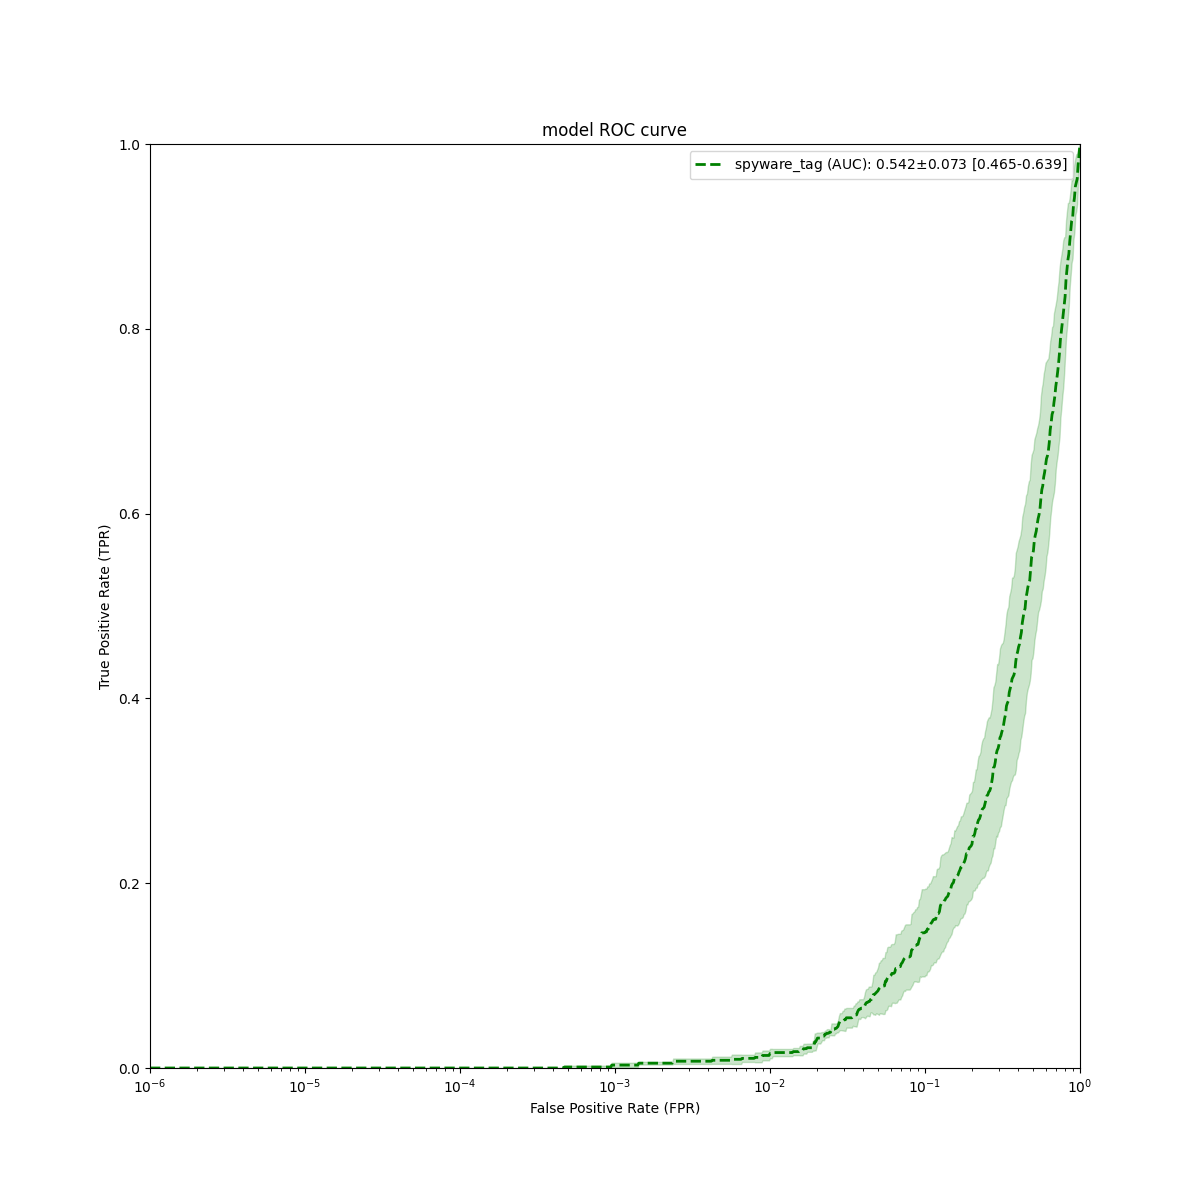
\includegraphics[width=0.6\textwidth]{./results/spyware_tag_roc_aloha.png}
        \vspace*{-0.2cm}
        \caption{ROC curve and AUC statistics of \textBF{ALOHA} model for the \textbf{Spyware Tag}. The line represents the \textit{mean} TPR at a given FPR, while the shaded region represents the \textit{standard deviation}. Statistics were computed over \textBF{3} training runs, each with random parameter initialization.}
        \label{fig:spywareTagRocAloha}
    \end{figure}
}

\newcommand{\spywareTagRocJointEmbedding}{
    \begin{figure}[H]
        \vspace*{-0.5cm}
        \centering
        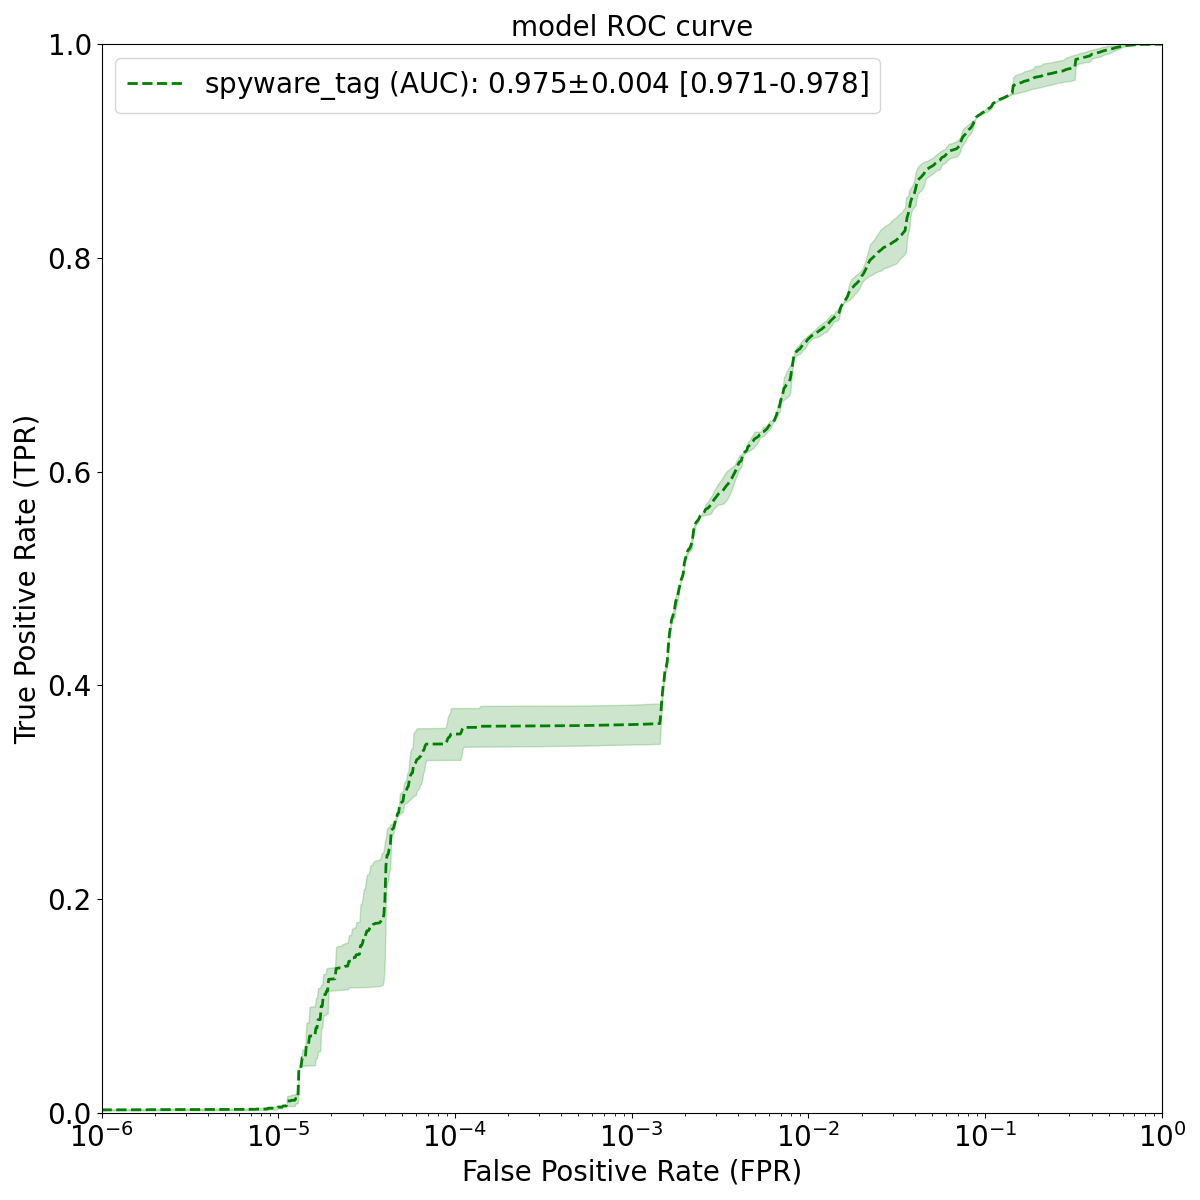
\includegraphics[width=0.6\textwidth]{./results/spyware_tag_roc_jointEmbedding.png}
        \vspace*{-0.2cm}
        \caption{ROC curve and AUC statistics of \textBF{Joint Embedding} model for the \textbf{Spyware Tag}. The line represents the \textit{mean} TPR at a given FPR, while the shaded region represents the \textit{standard deviation}. Statistics were computed over \textBF{3} training runs, each with random parameter initialization.}
        \label{fig:spywareTagRocJointEmbedding}
    \end{figure}
}

\newcommand{\spywareTagRocProposedMethod}{
    \begin{figure}[H]
        \vspace*{-0.5cm}
        \centering
        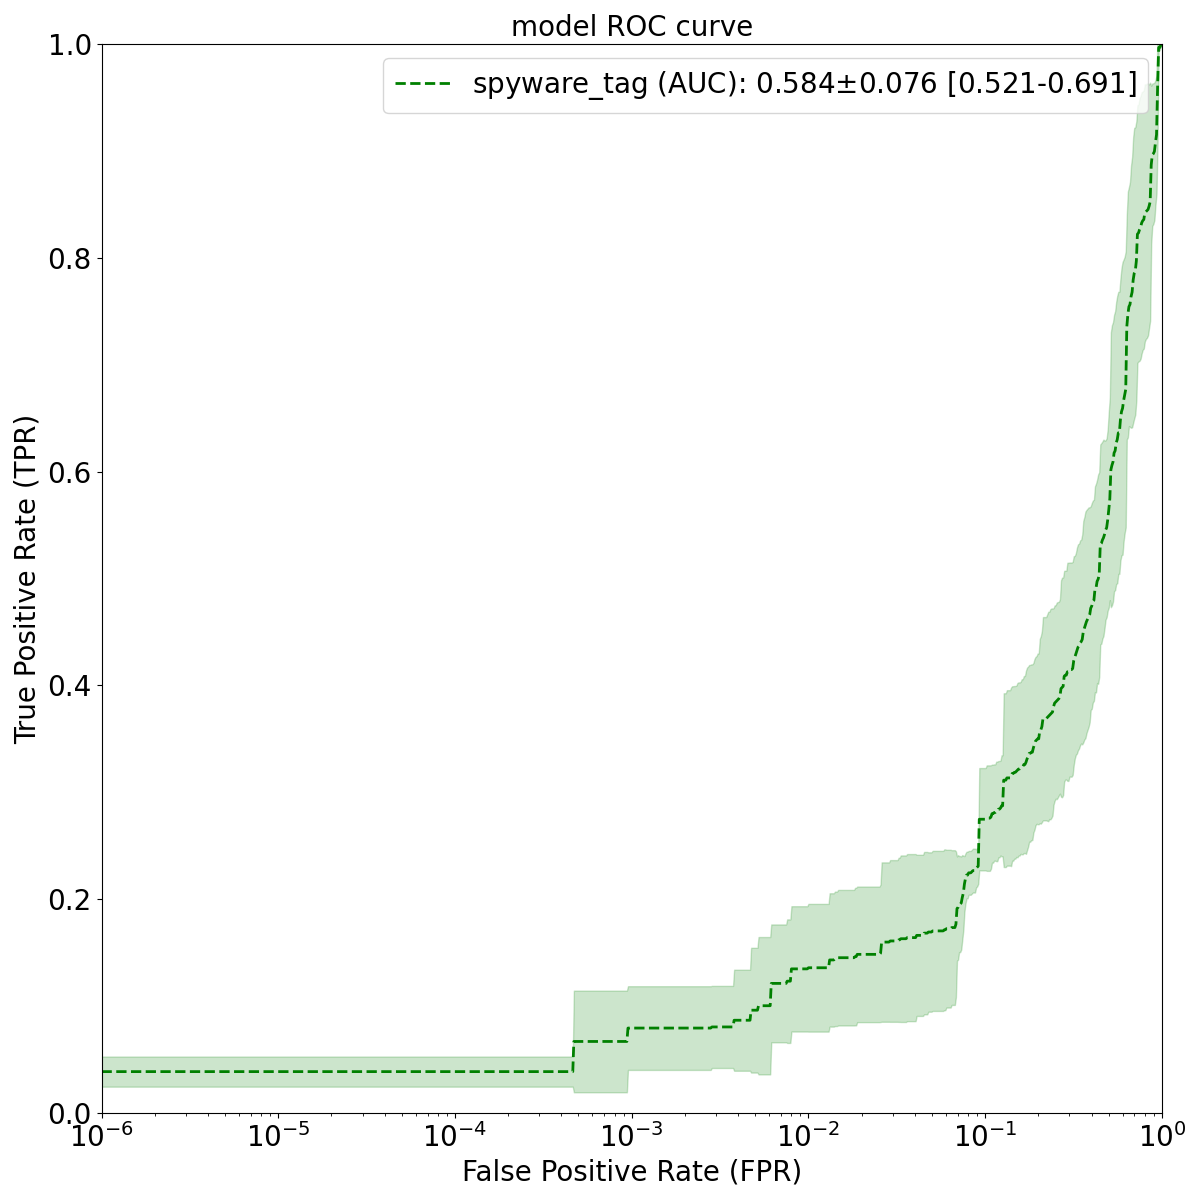
\includegraphics[width=0.6\textwidth]{./results/spyware_tag_roc_proposedModel.png}
        \vspace*{-0.2cm}
        \caption{ROC curve and AUC statistics of \textBF{Proposed Model} for the \textbf{Spyware Tag}. The line represents the \textit{mean} TPR at a given FPR, while the shaded region represents the \textit{standard deviation}. Statistics were computed over \textBF{3} training runs, each with random parameter initialization.}
        \label{fig:spywareTagRocProposedModel}
    \end{figure}
}
